\documentclass[1p]{elsarticle_modified}
%\bibliographystyle{elsarticle-num}

%\usepackage[colorlinks]{hyperref}
%\usepackage{abbrmath_seonhwa} %\Abb, \Ascr, \Acal ,\Abf, \Afrak
\usepackage{amsfonts}
\usepackage{amssymb}
\usepackage{amsmath}
\usepackage{amsthm}
\usepackage{scalefnt}
\usepackage{amsbsy}
\usepackage{kotex}
\usepackage{caption}
\usepackage{subfig}
\usepackage{color}
\usepackage{graphicx}
\usepackage{xcolor} %% white, black, red, green, blue, cyan, magenta, yellow
\usepackage{float}
\usepackage{setspace}
\usepackage{hyperref}

\usepackage{tikz}
\usetikzlibrary{arrows}

\usepackage{multirow}
\usepackage{array} % fixed length table
\usepackage{hhline}

%%%%%%%%%%%%%%%%%%%%%
\makeatletter
\renewcommand*\env@matrix[1][\arraystretch]{%
	\edef\arraystretch{#1}%
	\hskip -\arraycolsep
	\let\@ifnextchar\new@ifnextchar
	\array{*\c@MaxMatrixCols c}}
\makeatother %https://tex.stackexchange.com/questions/14071/how-can-i-increase-the-line-spacing-in-a-matrix
%%%%%%%%%%%%%%%

\usepackage[normalem]{ulem}

\newcommand{\msout}[1]{\ifmmode\text{\sout{\ensuremath{#1}}}\else\sout{#1}\fi}
%SOURCE: \msout is \stkout macro in https://tex.stackexchange.com/questions/20609/strikeout-in-math-mode

\newcommand{\cancel}[1]{
	\ifmmode
	{\color{red}\msout{#1}}
	\else
	{\color{red}\sout{#1}}
	\fi
}

\newcommand{\add}[1]{
	{\color{blue}\uwave{#1}}
}

\newcommand{\replace}[2]{
	\ifmmode
	{\color{red}\msout{#1}}{\color{blue}\uwave{#2}}
	\else
	{\color{red}\sout{#1}}{\color{blue}\uwave{#2}}
	\fi
}

\newcommand{\Sol}{\mathcal{S}} %segment
\newcommand{\D}{D} %diagram
\newcommand{\A}{\mathcal{A}} %arc


%%%%%%%%%%%%%%%%%%%%%%%%%%%%%5 test

\def\sl{\operatorname{\textup{SL}}(2,\Cbb)}
\def\psl{\operatorname{\textup{PSL}}(2,\Cbb)}
\def\quan{\mkern 1mu \triangleright \mkern 1mu}

\theoremstyle{definition}
\newtheorem{thm}{Theorem}[section]
\newtheorem{prop}[thm]{Proposition}
\newtheorem{lem}[thm]{Lemma}
\newtheorem{ques}[thm]{Question}
\newtheorem{cor}[thm]{Corollary}
\newtheorem{defn}[thm]{Definition}
\newtheorem{exam}[thm]{Example}
\newtheorem{rmk}[thm]{Remark}
\newtheorem{alg}[thm]{Algorithm}

\newcommand{\I}{\sqrt{-1}}
\begin{document}

%\begin{frontmatter}
%
%\title{Boundary parabolic representations of knots up to 8 crossings}
%
%%% Group authors per affiliation:
%\author{Yunhi Cho} 
%\address{Department of Mathematics, University of Seoul, Seoul, Korea}
%\ead{yhcho@uos.ac.kr}
%
%
%\author{Seonhwa Kim} %\fnref{s_kim}}
%\address{Center for Geometry and Physics, Institute for Basic Science, Pohang, 37673, Korea}
%\ead{ryeona17@ibs.re.kr}
%
%\author{Hyuk Kim}
%\address{Department of Mathematical Sciences, Seoul National University, Seoul 08826, Korea}
%\ead{hyukkim@snu.ac.kr}
%
%\author{Seokbeom Yoon}
%\address{Department of Mathematical Sciences, Seoul National University, Seoul, 08826,  Korea}
%\ead{sbyoon15@snu.ac.kr}
%
%\begin{abstract}
%We find all boundary parabolic representation of knots up to 8 crossings.
%
%\end{abstract}
%\begin{keyword}
%    \MSC[2010] 57M25 
%\end{keyword}
%
%\end{frontmatter}

%\linenumbers
%\tableofcontents
%
\newcommand\colored[1]{\textcolor{white}{\rule[-0.35ex]{0.8em}{1.4ex}}\kern-0.8em\color{red} #1}%
%\newcommand\colored[1]{\textcolor{white}{ #1}\kern-2.17ex	\textcolor{white}{ #1}\kern-1.81ex	\textcolor{white}{ #1}\kern-2.15ex\color{red}#1	}

{\Large $\underline{11a_{36}~(K11a_{36})}$}

\setlength{\tabcolsep}{10pt}
\renewcommand{\arraystretch}{1.6}
\vspace{1cm}\begin{tabular}{m{100pt}>{\centering\arraybackslash}m{274pt}}
\multirow{5}{120pt}{
	\centering
	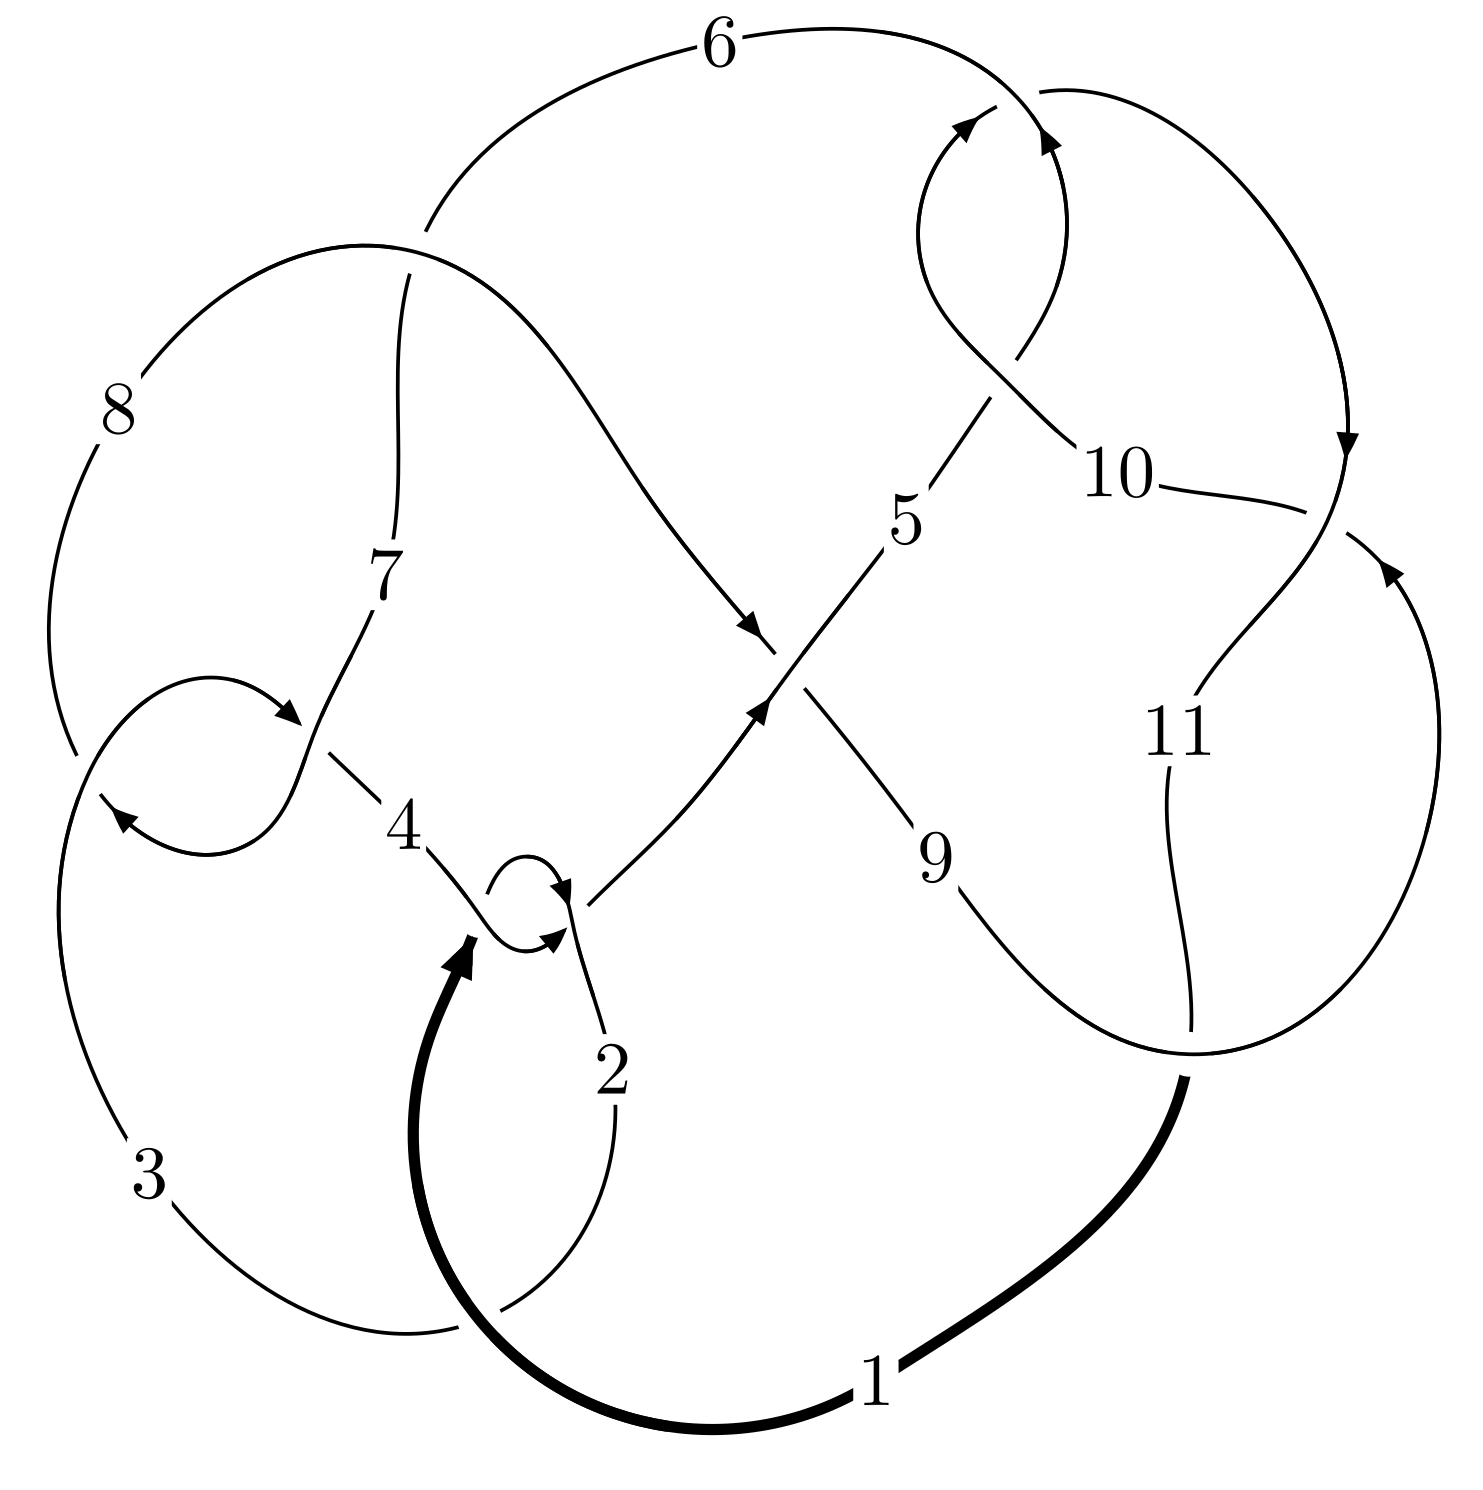
\includegraphics[width=112pt]{../../../GIT/diagram.site/Diagrams/png/285_11a_36.png}\\
\ \ \ A knot diagram\footnotemark}&
\allowdisplaybreaks
\textbf{Linearized knot diagam} \\
\cline{2-2}
 &
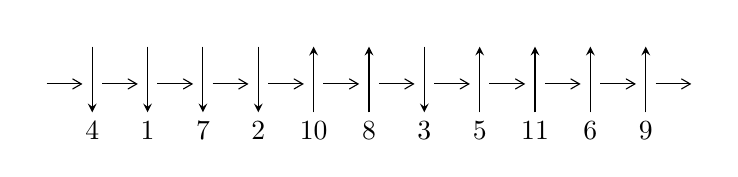
\begin{tikzpicture}[x=20pt, y=17pt]
	% nodes
	\node (C0) at (0, 0) {};
	\node (C1) at (1, 0) {};
	\node (C1U) at (1, +1) {};
	\node (C1D) at (1, -1) {4};

	\node (C2) at (2, 0) {};
	\node (C2U) at (2, +1) {};
	\node (C2D) at (2, -1) {1};

	\node (C3) at (3, 0) {};
	\node (C3U) at (3, +1) {};
	\node (C3D) at (3, -1) {7};

	\node (C4) at (4, 0) {};
	\node (C4U) at (4, +1) {};
	\node (C4D) at (4, -1) {2};

	\node (C5) at (5, 0) {};
	\node (C5U) at (5, +1) {};
	\node (C5D) at (5, -1) {10};

	\node (C6) at (6, 0) {};
	\node (C6U) at (6, +1) {};
	\node (C6D) at (6, -1) {8};

	\node (C7) at (7, 0) {};
	\node (C7U) at (7, +1) {};
	\node (C7D) at (7, -1) {3};

	\node (C8) at (8, 0) {};
	\node (C8U) at (8, +1) {};
	\node (C8D) at (8, -1) {5};

	\node (C9) at (9, 0) {};
	\node (C9U) at (9, +1) {};
	\node (C9D) at (9, -1) {11};

	\node (C10) at (10, 0) {};
	\node (C10U) at (10, +1) {};
	\node (C10D) at (10, -1) {6};

	\node (C11) at (11, 0) {};
	\node (C11U) at (11, +1) {};
	\node (C11D) at (11, -1) {9};
	\node (C12) at (12, 0) {};

	% arrows
	\draw[->,>={angle 60}]
	(C0) edge (C1) (C1) edge (C2) (C2) edge (C3) (C3) edge (C4) (C4) edge (C5) (C5) edge (C6) (C6) edge (C7) (C7) edge (C8) (C8) edge (C9) (C9) edge (C10) (C10) edge (C11) (C11) edge (C12) ;	\draw[->,>=stealth]
	(C1U) edge (C1D) (C2U) edge (C2D) (C3U) edge (C3D) (C4U) edge (C4D) (C5D) edge (C5U) (C6D) edge (C6U) (C7U) edge (C7D) (C8D) edge (C8U) (C9D) edge (C9U) (C10D) edge (C10U) (C11D) edge (C11U) ;
	\end{tikzpicture} \\
\hhline{~~} \\& 
\textbf{Solving Sequence} \\ \cline{2-2} 
 &
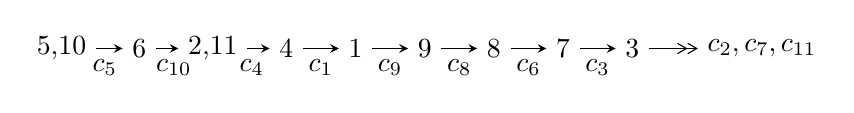
\begin{tikzpicture}[x=25pt, y=7pt]
	% node
	\node (A0) at (-1/8, 0) {5,10};
	\node (A1) at (1, 0) {6};
	\node (A2) at (33/16, 0) {2,11};
	\node (A3) at (25/8, 0) {4};
	\node (A4) at (33/8, 0) {1};
	\node (A5) at (41/8, 0) {9};
	\node (A6) at (49/8, 0) {8};
	\node (A7) at (57/8, 0) {7};
	\node (A8) at (65/8, 0) {3};
	\node (C1) at (1/2, -1) {$c_{5}$};
	\node (C2) at (3/2, -1) {$c_{10}$};
	\node (C3) at (21/8, -1) {$c_{4}$};
	\node (C4) at (29/8, -1) {$c_{1}$};
	\node (C5) at (37/8, -1) {$c_{9}$};
	\node (C6) at (45/8, -1) {$c_{8}$};
	\node (C7) at (53/8, -1) {$c_{6}$};
	\node (C8) at (61/8, -1) {$c_{3}$};
	\node (A9) at (10, 0) {$c_{2},c_{7},c_{11}$};

	% edge
	\draw[->,>=stealth]	
	(A0) edge (A1) (A1) edge (A2) (A2) edge (A3) (A3) edge (A4) (A4) edge (A5) (A5) edge (A6) (A6) edge (A7) (A7) edge (A8) ;
	\draw[->>,>={angle 60}]	
	(A8) edge (A9);
\end{tikzpicture} \\ 

\end{tabular} \\

\footnotetext{
The image of knot diagram is generated by the software ``\textbf{Draw programme}" developed by Andrew Bartholomew(\url{http://www.layer8.co.uk/maths/draw/index.htm\#Running-draw}), where we modified some parts for our purpose(\url{https://github.com/CATsTAILs/LinksPainter}).
}\phantom \\ \newline 
\centering \textbf{Ideals for irreducible components\footnotemark of $X_{\text{par}}$} 
 
\begin{align*}
I^u_{1}&=\langle 
u^{62}- u^{61}+\cdots+b-2 u,\;- u^{60}+u^{59}+\cdots+a-2,\;u^{63}-2 u^{62}+\cdots-10 u^2+1\rangle \\
I^u_{2}&=\langle 
b+1,\;a+u,\;u^3- u^2+1\rangle \\
\\
\end{align*}
\raggedright * 2 irreducible components of $\dim_{\mathbb{C}}=0$, with total 66 representations.\\
\footnotetext{All coefficients of polynomials are rational numbers. But the coefficients are sometimes approximated in decimal forms when there is not enough margin.}
\newpage
\renewcommand{\arraystretch}{1}
\centering \section*{I. $I^u_{1}= \langle u^{62}- u^{61}+\cdots+b-2 u,\;- u^{60}+u^{59}+\cdots+a-2,\;u^{63}-2 u^{62}+\cdots-10 u^2+1 \rangle$}
\flushleft \textbf{(i) Arc colorings}\\
\begin{tabular}{m{7pt} m{180pt} m{7pt} m{180pt} }
\flushright $a_{5}=$&$\begin{pmatrix}1\\0\end{pmatrix}$ \\
\flushright $a_{10}=$&$\begin{pmatrix}0\\u\end{pmatrix}$ \\
\flushright $a_{6}=$&$\begin{pmatrix}1\\- u^2\end{pmatrix}$ \\
\flushright $a_{2}=$&$\begin{pmatrix}u^{60}- u^{59}+\cdots-4 u+2\\- u^{62}+u^{61}+\cdots-6 u^2+2 u\end{pmatrix}$ \\
\flushright $a_{11}=$&$\begin{pmatrix}u\\- u^3+u\end{pmatrix}$ \\
\flushright $a_{4}=$&$\begin{pmatrix}- u^{62}+u^{61}+\cdots-4 u+3\\- u^{62}+u^{61}+\cdots-7 u^2+u\end{pmatrix}$ \\
\flushright $a_{1}=$&$\begin{pmatrix}u^5+u\\- u^7+u^5-2 u^3+u\end{pmatrix}$ \\
\flushright $a_{9}=$&$\begin{pmatrix}- u^3\\u^5- u^3+u\end{pmatrix}$ \\
\flushright $a_{8}=$&$\begin{pmatrix}- u^5- u\\u^5- u^3+u\end{pmatrix}$ \\
\flushright $a_{7}=$&$\begin{pmatrix}- u^{12}+u^{10}-3 u^8+2 u^6-2 u^4+u^2+1\\u^{12}-2 u^{10}+4 u^8-4 u^6+3 u^4-2 u^2\end{pmatrix}$ \\
\flushright $a_{3}=$&$\begin{pmatrix}u^{62}- u^{61}+\cdots-4 u+2\\- u^{62}+u^{61}+\cdots-5 u^2+2 u\end{pmatrix}$\\ \flushright $a_{3}=$&$\begin{pmatrix}u^{62}- u^{61}+\cdots-4 u+2\\- u^{62}+u^{61}+\cdots-5 u^2+2 u\end{pmatrix}$\\&\end{tabular}
\flushleft \textbf{(ii) Obstruction class $= -1$}\\~\\
\flushleft \textbf{(iii) Cusp Shapes $= -11 u^{62}+14 u^{61}+\cdots+25 u+5$}\\~\\
\newpage\renewcommand{\arraystretch}{1}
\flushleft \textbf{(iv) u-Polynomials at the component}\newline \\
\begin{tabular}{m{50pt}|m{274pt}}
Crossings & \hspace{64pt}u-Polynomials at each crossing \\
\hline $$\begin{aligned}c_{1},c_{4}\end{aligned}$$&$\begin{aligned}
&u^{63}-4 u^{62}+\cdots-3 u+1
\end{aligned}$\\
\hline $$\begin{aligned}c_{2}\end{aligned}$$&$\begin{aligned}
&u^{63}+34 u^{62}+\cdots+5 u+1
\end{aligned}$\\
\hline $$\begin{aligned}c_{3},c_{7}\end{aligned}$$&$\begin{aligned}
&u^{63}+u^{62}+\cdots+12 u+8
\end{aligned}$\\
\hline $$\begin{aligned}c_{5},c_{10}\end{aligned}$$&$\begin{aligned}
&u^{63}-2 u^{62}+\cdots-10 u^2+1
\end{aligned}$\\
\hline $$\begin{aligned}c_{6}\end{aligned}$$&$\begin{aligned}
&u^{63}-21 u^{62}+\cdots-624 u+64
\end{aligned}$\\
\hline $$\begin{aligned}c_{8}\end{aligned}$$&$\begin{aligned}
&u^{63}+2 u^{62}+\cdots-18 u+9
\end{aligned}$\\
\hline $$\begin{aligned}c_{9},c_{11}\end{aligned}$$&$\begin{aligned}
&u^{63}-20 u^{62}+\cdots+20 u-1
\end{aligned}$\\
\hline
\end{tabular}\\~\\
\newpage\renewcommand{\arraystretch}{1}
\flushleft \textbf{(v) Riley Polynomials at the component}\newline \\
\begin{tabular}{m{50pt}|m{274pt}}
Crossings & \hspace{64pt}Riley Polynomials at each crossing \\
\hline $$\begin{aligned}c_{1},c_{4}\end{aligned}$$&$\begin{aligned}
&y^{63}-34 y^{62}+\cdots+5 y-1
\end{aligned}$\\
\hline $$\begin{aligned}c_{2}\end{aligned}$$&$\begin{aligned}
&y^{63}-6 y^{62}+\cdots-27 y-1
\end{aligned}$\\
\hline $$\begin{aligned}c_{3},c_{7}\end{aligned}$$&$\begin{aligned}
&y^{63}+21 y^{62}+\cdots-624 y-64
\end{aligned}$\\
\hline $$\begin{aligned}c_{5},c_{10}\end{aligned}$$&$\begin{aligned}
&y^{63}-20 y^{62}+\cdots+20 y-1
\end{aligned}$\\
\hline $$\begin{aligned}c_{6}\end{aligned}$$&$\begin{aligned}
&y^{63}+37 y^{62}+\cdots+167168 y-4096
\end{aligned}$\\
\hline $$\begin{aligned}c_{8}\end{aligned}$$&$\begin{aligned}
&y^{63}+12 y^{62}+\cdots-16272 y-81
\end{aligned}$\\
\hline $$\begin{aligned}c_{9},c_{11}\end{aligned}$$&$\begin{aligned}
&y^{63}+48 y^{62}+\cdots+340 y-1
\end{aligned}$\\
\hline
\end{tabular}\\~\\
\newpage\flushleft \textbf{(vi) Complex Volumes and Cusp Shapes}
$$\begin{array}{c|c|c}  
\text{Solutions to }I^u_{1}& \I (\text{vol} + \sqrt{-1}CS) & \text{Cusp shape}\\
 \hline 
\begin{aligned}
u &= \phantom{-}0.986745 + 0.175564 I \\
a &= \phantom{-}0.61504 - 2.83433 I \\
b &= -1.081170 + 0.440014 I\end{aligned}
 & -0.60605 + 3.69700 I & \phantom{-}2.17014 - 4.90316 I \\ \hline\begin{aligned}
u &= \phantom{-}0.986745 - 0.175564 I \\
a &= \phantom{-}0.61504 + 2.83433 I \\
b &= -1.081170 - 0.440014 I\end{aligned}
 & -0.60605 - 3.69700 I & \phantom{-}2.17014 + 4.90316 I \\ \hline\begin{aligned}
u &= \phantom{-}0.874745 + 0.474777 I \\
a &= \phantom{-}0.286938 + 1.257720 I \\
b &= \phantom{-}0.415444 - 0.641775 I\end{aligned}
 & \phantom{-}1.88400 + 1.11201 I & \phantom{-}5.93092 - 2.67876 I \\ \hline\begin{aligned}
u &= \phantom{-}0.874745 - 0.474777 I \\
a &= \phantom{-}0.286938 - 1.257720 I \\
b &= \phantom{-}0.415444 + 0.641775 I\end{aligned}
 & \phantom{-}1.88400 - 1.11201 I & \phantom{-}5.93092 + 2.67876 I \\ \hline\begin{aligned}
u &= \phantom{-}0.964494 + 0.355493 I \\
a &= -0.902672 - 0.260134 I \\
b &= \phantom{-}1.089750 + 0.505160 I\end{aligned}
 & -0.13818 - 3.33082 I & \phantom{-}2.52685 + 2.17772 I \\ \hline\begin{aligned}
u &= \phantom{-}0.964494 - 0.355493 I \\
a &= -0.902672 + 0.260134 I \\
b &= \phantom{-}1.089750 - 0.505160 I\end{aligned}
 & -0.13818 + 3.33082 I & \phantom{-}2.52685 - 2.17772 I \\ \hline\begin{aligned}
u &= -0.812502 + 0.632834 I \\
a &= \phantom{-}0.90804 - 1.10283 I \\
b &= -0.817947 + 0.392240 I\end{aligned}
 & -2.19626 - 0.72911 I & \phantom{-0.000000 } 0 \\ \hline\begin{aligned}
u &= -0.812502 - 0.632834 I \\
a &= \phantom{-}0.90804 + 1.10283 I \\
b &= -0.817947 - 0.392240 I\end{aligned}
 & -2.19626 + 0.72911 I & \phantom{-0.000000 } 0 \\ \hline\begin{aligned}
u &= -1.028670 + 0.156882 I \\
a &= -1.00602 + 1.41426 I \\
b &= \phantom{-}0.264864 - 0.800811 I\end{aligned}
 & \phantom{-}3.55985 - 4.49777 I & \phantom{-}7.47027 + 4.85592 I \\ \hline\begin{aligned}
u &= -1.028670 - 0.156882 I \\
a &= -1.00602 - 1.41426 I \\
b &= \phantom{-}0.264864 + 0.800811 I\end{aligned}
 & \phantom{-}3.55985 + 4.49777 I & \phantom{-}7.47027 - 4.85592 I\\
 \hline 
 \end{array}$$\newpage$$\begin{array}{c|c|c}  
\text{Solutions to }I^u_{1}& \I (\text{vol} + \sqrt{-1}CS) & \text{Cusp shape}\\
 \hline 
\begin{aligned}
u &= -1.042190 + 0.029758 I \\
a &= -1.18918 - 2.02036 I \\
b &= \phantom{-}0.778473 + 0.655233 I\end{aligned}
 & \phantom{-}6.20929 - 2.51179 I & \phantom{-}9.63450 + 3.63863 I \\ \hline\begin{aligned}
u &= -1.042190 - 0.029758 I \\
a &= -1.18918 + 2.02036 I \\
b &= \phantom{-}0.778473 - 0.655233 I\end{aligned}
 & \phantom{-}6.20929 + 2.51179 I & \phantom{-}9.63450 - 3.63863 I \\ \hline\begin{aligned}
u &= -0.935551 + 0.179164 I \\
a &= \phantom{-}0.853660 - 0.118464 I \\
b &= -1.182530 + 0.257010 I\end{aligned}
 & -1.01619 - 1.23564 I & \phantom{-}2.18804 + 4.79371 I \\ \hline\begin{aligned}
u &= -0.935551 - 0.179164 I \\
a &= \phantom{-}0.853660 + 0.118464 I \\
b &= -1.182530 - 0.257010 I\end{aligned}
 & -1.01619 + 1.23564 I & \phantom{-}2.18804 - 4.79371 I \\ \hline\begin{aligned}
u &= -1.052700 + 0.191629 I \\
a &= -0.51296 - 2.42316 I \\
b &= \phantom{-}1.157220 + 0.552536 I\end{aligned}
 & \phantom{-}0.91945 - 9.52832 I & \phantom{-0.000000 -}0. + 8.35881 I \\ \hline\begin{aligned}
u &= -1.052700 - 0.191629 I \\
a &= -0.51296 + 2.42316 I \\
b &= \phantom{-}1.157220 - 0.552536 I\end{aligned}
 & \phantom{-}0.91945 + 9.52832 I & \phantom{-0.000000 } 0. - 8.35881 I \\ \hline\begin{aligned}
u &= \phantom{-}0.708953 + 0.814144 I \\
a &= -0.019906 + 0.202917 I \\
b &= \phantom{-}0.178721 - 0.848670 I\end{aligned}
 & -2.92774 - 4.17173 I & \phantom{-0.000000 } 0 \\ \hline\begin{aligned}
u &= \phantom{-}0.708953 - 0.814144 I \\
a &= -0.019906 - 0.202917 I \\
b &= \phantom{-}0.178721 + 0.848670 I\end{aligned}
 & -2.92774 + 4.17173 I & \phantom{-0.000000 } 0 \\ \hline\begin{aligned}
u &= \phantom{-}0.607392 + 0.688668 I \\
a &= \phantom{-}0.119031 - 0.627685 I \\
b &= \phantom{-}0.881881 + 0.575730 I\end{aligned}
 & \phantom{-}0.93068 - 3.11451 I & \phantom{-}1.81708 + 3.79797 I \\ \hline\begin{aligned}
u &= \phantom{-}0.607392 - 0.688668 I \\
a &= \phantom{-}0.119031 + 0.627685 I \\
b &= \phantom{-}0.881881 - 0.575730 I\end{aligned}
 & \phantom{-}0.93068 + 3.11451 I & \phantom{-}1.81708 - 3.79797 I\\
 \hline 
 \end{array}$$\newpage$$\begin{array}{c|c|c}  
\text{Solutions to }I^u_{1}& \I (\text{vol} + \sqrt{-1}CS) & \text{Cusp shape}\\
 \hline 
\begin{aligned}
u &= -0.730831 + 0.812085 I \\
a &= -1.03790 - 0.99175 I \\
b &= -1.158560 + 0.468666 I\end{aligned}
 & -7.07861 + 2.97979 I & \phantom{-0.000000 } 0 \\ \hline\begin{aligned}
u &= -0.730831 - 0.812085 I \\
a &= -1.03790 + 0.99175 I \\
b &= -1.158560 - 0.468666 I\end{aligned}
 & -7.07861 - 2.97979 I & \phantom{-0.000000 } 0 \\ \hline\begin{aligned}
u &= \phantom{-}0.866834 + 0.666035 I \\
a &= -0.97074 - 1.07449 I \\
b &= -1.210370 + 0.030629 I\end{aligned}
 & -3.42806 + 2.58129 I & \phantom{-0.000000 } 0 \\ \hline\begin{aligned}
u &= \phantom{-}0.866834 - 0.666035 I \\
a &= -0.97074 + 1.07449 I \\
b &= -1.210370 - 0.030629 I\end{aligned}
 & -3.42806 - 2.58129 I & \phantom{-0.000000 } 0 \\ \hline\begin{aligned}
u &= -0.766973 + 0.785827 I \\
a &= \phantom{-}0.238443 + 0.199801 I \\
b &= -0.074618 - 0.675215 I\end{aligned}
 & -4.03831 - 1.31004 I & \phantom{-0.000000 } 0 \\ \hline\begin{aligned}
u &= -0.766973 - 0.785827 I \\
a &= \phantom{-}0.238443 - 0.199801 I \\
b &= -0.074618 + 0.675215 I\end{aligned}
 & -4.03831 + 1.31004 I & \phantom{-0.000000 } 0 \\ \hline\begin{aligned}
u &= \phantom{-}0.746245 + 0.806063 I \\
a &= -1.32268 - 0.61068 I \\
b &= -1.246680 + 0.342536 I\end{aligned}
 & -7.36657 - 0.17993 I & \phantom{-0.000000 } 0 \\ \hline\begin{aligned}
u &= \phantom{-}0.746245 - 0.806063 I \\
a &= -1.32268 + 0.61068 I \\
b &= -1.246680 - 0.342536 I\end{aligned}
 & -7.36657 + 0.17993 I & \phantom{-0.000000 } 0 \\ \hline\begin{aligned}
u &= \phantom{-}0.709456 + 0.839598 I \\
a &= \phantom{-}1.007390 - 0.709259 I \\
b &= \phantom{-}1.198760 + 0.538883 I\end{aligned}
 & -5.96644 - 9.24715 I & \phantom{-0.000000 } 0 \\ \hline\begin{aligned}
u &= \phantom{-}0.709456 - 0.839598 I \\
a &= \phantom{-}1.007390 + 0.709259 I \\
b &= \phantom{-}1.198760 - 0.538883 I\end{aligned}
 & -5.96644 + 9.24715 I & \phantom{-0.000000 } 0\\
 \hline 
 \end{array}$$\newpage$$\begin{array}{c|c|c}  
\text{Solutions to }I^u_{1}& \I (\text{vol} + \sqrt{-1}CS) & \text{Cusp shape}\\
 \hline 
\begin{aligned}
u &= \phantom{-}0.896870 + 0.059236 I \\
a &= \phantom{-}1.60096 + 0.91476 I \\
b &= -0.331068 - 0.319832 I\end{aligned}
 & \phantom{-}1.55408 + 0.10582 I & \phantom{-}6.26556 + 0.58371 I \\ \hline\begin{aligned}
u &= \phantom{-}0.896870 - 0.059236 I \\
a &= \phantom{-}1.60096 - 0.91476 I \\
b &= -0.331068 + 0.319832 I\end{aligned}
 & \phantom{-}1.55408 - 0.10582 I & \phantom{-}6.26556 - 0.58371 I \\ \hline\begin{aligned}
u &= -0.915129 + 0.657239 I \\
a &= \phantom{-}0.50428 + 2.10750 I \\
b &= -0.706877 - 0.424114 I\end{aligned}
 & -1.85739 - 4.32227 I & \phantom{-0.000000 } 0 \\ \hline\begin{aligned}
u &= -0.915129 - 0.657239 I \\
a &= \phantom{-}0.50428 - 2.10750 I \\
b &= -0.706877 + 0.424114 I\end{aligned}
 & -1.85739 + 4.32227 I & \phantom{-0.000000 } 0 \\ \hline\begin{aligned}
u &= -0.788679 + 0.828583 I \\
a &= \phantom{-}1.248600 - 0.560983 I \\
b &= \phantom{-}1.153780 + 0.425567 I\end{aligned}
 & -7.38822 - 5.19388 I & \phantom{-0.000000 } 0 \\ \hline\begin{aligned}
u &= -0.788679 - 0.828583 I \\
a &= \phantom{-}1.248600 + 0.560983 I \\
b &= \phantom{-}1.153780 - 0.425567 I\end{aligned}
 & -7.38822 + 5.19388 I & \phantom{-0.000000 } 0 \\ \hline\begin{aligned}
u &= \phantom{-}0.972413 + 0.616521 I \\
a &= -1.155960 - 0.419026 I \\
b &= \phantom{-}0.638145 + 0.682574 I\end{aligned}
 & \phantom{-}2.75209 + 3.26890 I & \phantom{-0.000000 } 0 \\ \hline\begin{aligned}
u &= \phantom{-}0.972413 - 0.616521 I \\
a &= -1.155960 + 0.419026 I \\
b &= \phantom{-}0.638145 - 0.682574 I\end{aligned}
 & \phantom{-}2.75209 - 3.26890 I & \phantom{-0.000000 } 0 \\ \hline\begin{aligned}
u &= -0.880612 + 0.777007 I \\
a &= \phantom{-}0.870304 - 0.514339 I \\
b &= \phantom{-}0.742658 + 0.034260 I\end{aligned}
 & -3.99010 - 2.92514 I & \phantom{-0.000000 } 0 \\ \hline\begin{aligned}
u &= -0.880612 - 0.777007 I \\
a &= \phantom{-}0.870304 + 0.514339 I \\
b &= \phantom{-}0.742658 - 0.034260 I\end{aligned}
 & -3.99010 + 2.92514 I & \phantom{-0.000000 } 0\\
 \hline 
 \end{array}$$\newpage$$\begin{array}{c|c|c}  
\text{Solutions to }I^u_{1}& \I (\text{vol} + \sqrt{-1}CS) & \text{Cusp shape}\\
 \hline 
\begin{aligned}
u &= \phantom{-}0.995425 + 0.656387 I \\
a &= \phantom{-}0.43151 + 2.20348 I \\
b &= \phantom{-}0.892480 - 0.637862 I\end{aligned}
 & \phantom{-}2.02729 + 8.31052 I & \phantom{-0.000000 } 0 \\ \hline\begin{aligned}
u &= \phantom{-}0.995425 - 0.656387 I \\
a &= \phantom{-}0.43151 - 2.20348 I \\
b &= \phantom{-}0.892480 + 0.637862 I\end{aligned}
 & \phantom{-}2.02729 - 8.31052 I & \phantom{-0.000000 } 0 \\ \hline\begin{aligned}
u &= -0.963455 + 0.732228 I \\
a &= \phantom{-}1.199630 - 0.298215 I \\
b &= -0.136404 + 0.659647 I\end{aligned}
 & -3.43377 - 4.42046 I & \phantom{-0.000000 } 0 \\ \hline\begin{aligned}
u &= -0.963455 - 0.732228 I \\
a &= \phantom{-}1.199630 + 0.298215 I \\
b &= -0.136404 - 0.659647 I\end{aligned}
 & -3.43377 + 4.42046 I & \phantom{-0.000000 } 0 \\ \hline\begin{aligned}
u &= \phantom{-}0.982283 + 0.738862 I \\
a &= -0.457935 - 0.943864 I \\
b &= -1.260650 - 0.325376 I\end{aligned}
 & -6.64299 + 5.98946 I & \phantom{-0.000000 } 0 \\ \hline\begin{aligned}
u &= \phantom{-}0.982283 - 0.738862 I \\
a &= -0.457935 + 0.943864 I \\
b &= -1.260650 + 0.325376 I\end{aligned}
 & -6.64299 - 5.98946 I & \phantom{-0.000000 } 0 \\ \hline\begin{aligned}
u &= -0.965072 + 0.771283 I \\
a &= \phantom{-}0.443626 - 0.814250 I \\
b &= \phantom{-}1.141120 - 0.407113 I\end{aligned}
 & -6.84424 - 0.78588 I & \phantom{-0.000000 } 0 \\ \hline\begin{aligned}
u &= -0.965072 - 0.771283 I \\
a &= \phantom{-}0.443626 + 0.814250 I \\
b &= \phantom{-}1.141120 + 0.407113 I\end{aligned}
 & -6.84424 + 0.78588 I & \phantom{-0.000000 } 0 \\ \hline\begin{aligned}
u &= -0.992955 + 0.736861 I \\
a &= -1.15889 + 2.64082 I \\
b &= -1.148080 - 0.485998 I\end{aligned}
 & -6.27660 - 8.79934 I & \phantom{-0.000000 } 0 \\ \hline\begin{aligned}
u &= -0.992955 - 0.736861 I \\
a &= -1.15889 - 2.64082 I \\
b &= -1.148080 + 0.485998 I\end{aligned}
 & -6.27660 + 8.79934 I & \phantom{-0.000000 } 0\\
 \hline 
 \end{array}$$\newpage$$\begin{array}{c|c|c}  
\text{Solutions to }I^u_{1}& \I (\text{vol} + \sqrt{-1}CS) & \text{Cusp shape}\\
 \hline 
\begin{aligned}
u &= \phantom{-}1.004710 + 0.730240 I \\
a &= -1.188500 - 0.320665 I \\
b &= \phantom{-}0.198021 + 0.868774 I\end{aligned}
 & -2.02603 + 9.97382 I & \phantom{-0.000000 } 0 \\ \hline\begin{aligned}
u &= \phantom{-}1.004710 - 0.730240 I \\
a &= -1.188500 + 0.320665 I \\
b &= \phantom{-}0.198021 - 0.868774 I\end{aligned}
 & -2.02603 - 9.97382 I & \phantom{-0.000000 } 0 \\ \hline\begin{aligned}
u &= \phantom{-}1.014130 + 0.742144 I \\
a &= \phantom{-}1.18770 + 2.38163 I \\
b &= \phantom{-}1.201630 - 0.551168 I\end{aligned}
 & -5.0319 + 15.1597 I & \phantom{-0.000000 } 0 \\ \hline\begin{aligned}
u &= \phantom{-}1.014130 - 0.742144 I \\
a &= \phantom{-}1.18770 - 2.38163 I \\
b &= \phantom{-}1.201630 + 0.551168 I\end{aligned}
 & -5.0319 - 15.1597 I & \phantom{-0.000000 } 0 \\ \hline\begin{aligned}
u &= \phantom{-}0.467397 + 0.552241 I \\
a &= \phantom{-}0.336545 + 0.777590 I \\
b &= \phantom{-}0.656494 - 0.538703 I\end{aligned}
 & \phantom{-}1.61397 + 1.37996 I & \phantom{-}3.33026 - 3.84355 I \\ \hline\begin{aligned}
u &= \phantom{-}0.467397 - 0.552241 I \\
a &= \phantom{-}0.336545 - 0.777590 I \\
b &= \phantom{-}0.656494 + 0.538703 I\end{aligned}
 & \phantom{-}1.61397 - 1.37996 I & \phantom{-}3.33026 + 3.84355 I \\ \hline\begin{aligned}
u &= \phantom{-}0.100658 + 0.672094 I \\
a &= \phantom{-}1.138600 + 0.751362 I \\
b &= \phantom{-}1.149530 - 0.509940 I\end{aligned}
 & -2.82669 + 6.78405 I & -3.37376 - 6.18383 I \\ \hline\begin{aligned}
u &= \phantom{-}0.100658 - 0.672094 I \\
a &= \phantom{-}1.138600 - 0.751362 I \\
b &= \phantom{-}1.149530 + 0.509940 I\end{aligned}
 & -2.82669 - 6.78405 I & -3.37376 + 6.18383 I \\ \hline\begin{aligned}
u &= \phantom{-}0.126664 + 0.583968 I \\
a &= \phantom{-}0.0087736 - 0.0534979 I \\
b &= \phantom{-}0.195316 + 0.700814 I\end{aligned}
 & -0.08935 + 2.18002 I & -0.08533 - 3.20984 I \\ \hline\begin{aligned}
u &= \phantom{-}0.126664 - 0.583968 I \\
a &= \phantom{-}0.0087736 + 0.0534979 I \\
b &= \phantom{-}0.195316 - 0.700814 I\end{aligned}
 & -0.08935 - 2.18002 I & -0.08533 + 3.20984 I\\
 \hline 
 \end{array}$$\newpage$$\begin{array}{c|c|c}  
\text{Solutions to }I^u_{1}& \I (\text{vol} + \sqrt{-1}CS) & \text{Cusp shape}\\
 \hline 
\begin{aligned}
u &= -0.032116 + 0.576226 I \\
a &= -1.38838 + 1.00826 I \\
b &= -1.143910 - 0.371905 I\end{aligned}
 & -3.80293 - 1.26646 I & -5.80106 + 0.80985 I \\ \hline\begin{aligned}
u &= -0.032116 - 0.576226 I \\
a &= -1.38838 - 1.00826 I \\
b &= -1.143910 + 0.371905 I\end{aligned}
 & -3.80293 + 1.26646 I & -5.80106 - 0.80985 I \\ \hline\begin{aligned}
u &= -0.235960\phantom{ +0.000000I} \\
a &= \phantom{-}2.62532\phantom{ +0.000000I} \\
b &= -0.870881\phantom{ +0.000000I}\end{aligned}
 & -1.26098\phantom{ +0.000000I} & -8.95540\phantom{ +0.000000I}\\
 \hline 
 \end{array}$$\newpage\newpage\renewcommand{\arraystretch}{1}
\centering \section*{II. $I^u_{2}= \langle b+1,\;a+u,\;u^3- u^2+1 \rangle$}
\flushleft \textbf{(i) Arc colorings}\\
\begin{tabular}{m{7pt} m{180pt} m{7pt} m{180pt} }
\flushright $a_{5}=$&$\begin{pmatrix}1\\0\end{pmatrix}$ \\
\flushright $a_{10}=$&$\begin{pmatrix}0\\u\end{pmatrix}$ \\
\flushright $a_{6}=$&$\begin{pmatrix}1\\- u^2\end{pmatrix}$ \\
\flushright $a_{2}=$&$\begin{pmatrix}- u\\-1\end{pmatrix}$ \\
\flushright $a_{11}=$&$\begin{pmatrix}u\\- u^2+u+1\end{pmatrix}$ \\
\flushright $a_{4}=$&$\begin{pmatrix}- u+1\\-1\end{pmatrix}$ \\
\flushright $a_{1}=$&$\begin{pmatrix}-1\\0\end{pmatrix}$ \\
\flushright $a_{9}=$&$\begin{pmatrix}- u^2+1\\- u^2\end{pmatrix}$ \\
\flushright $a_{8}=$&$\begin{pmatrix}1\\- u^2\end{pmatrix}$ \\
\flushright $a_{7}=$&$\begin{pmatrix}1\\- u^2\end{pmatrix}$ \\
\flushright $a_{3}=$&$\begin{pmatrix}- u+1\\-1\end{pmatrix}$\\ \flushright $a_{3}=$&$\begin{pmatrix}- u+1\\-1\end{pmatrix}$\\&\end{tabular}
\flushleft \textbf{(ii) Obstruction class $= 1$}\\~\\
\flushleft \textbf{(iii) Cusp Shapes $= 2 u^2-7 u-2$}\\~\\
\newpage\renewcommand{\arraystretch}{1}
\flushleft \textbf{(iv) u-Polynomials at the component}\newline \\
\begin{tabular}{m{50pt}|m{274pt}}
Crossings & \hspace{64pt}u-Polynomials at each crossing \\
\hline $$\begin{aligned}c_{1}\end{aligned}$$&$\begin{aligned}
&(u-1)^3
\end{aligned}$\\
\hline $$\begin{aligned}c_{2},c_{4}\end{aligned}$$&$\begin{aligned}
&(u+1)^3
\end{aligned}$\\
\hline $$\begin{aligned}c_{3},c_{6},c_{7}\end{aligned}$$&$\begin{aligned}
&u^3
\end{aligned}$\\
\hline $$\begin{aligned}c_{5}\end{aligned}$$&$\begin{aligned}
&u^3- u^2+1
\end{aligned}$\\
\hline $$\begin{aligned}c_{8},c_{11}\end{aligned}$$&$\begin{aligned}
&u^3- u^2+2 u-1
\end{aligned}$\\
\hline $$\begin{aligned}c_{9}\end{aligned}$$&$\begin{aligned}
&u^3+u^2+2 u+1
\end{aligned}$\\
\hline $$\begin{aligned}c_{10}\end{aligned}$$&$\begin{aligned}
&u^3+u^2-1
\end{aligned}$\\
\hline
\end{tabular}\\~\\
\newpage\renewcommand{\arraystretch}{1}
\flushleft \textbf{(v) Riley Polynomials at the component}\newline \\
\begin{tabular}{m{50pt}|m{274pt}}
Crossings & \hspace{64pt}Riley Polynomials at each crossing \\
\hline $$\begin{aligned}c_{1},c_{2},c_{4}\end{aligned}$$&$\begin{aligned}
&(y-1)^3
\end{aligned}$\\
\hline $$\begin{aligned}c_{3},c_{6},c_{7}\end{aligned}$$&$\begin{aligned}
&y^3
\end{aligned}$\\
\hline $$\begin{aligned}c_{5},c_{10}\end{aligned}$$&$\begin{aligned}
&y^3- y^2+2 y-1
\end{aligned}$\\
\hline $$\begin{aligned}c_{8},c_{9},c_{11}\end{aligned}$$&$\begin{aligned}
&y^3+3 y^2+2 y-1
\end{aligned}$\\
\hline
\end{tabular}\\~\\
\newpage\flushleft \textbf{(vi) Complex Volumes and Cusp Shapes}
$$\begin{array}{c|c|c}  
\text{Solutions to }I^u_{2}& \I (\text{vol} + \sqrt{-1}CS) & \text{Cusp shape}\\
 \hline 
\begin{aligned}
u &= \phantom{-}0.877439 + 0.744862 I \\
a &= -0.877439 - 0.744862 I \\
b &= -1.00000\phantom{ +0.000000I}\end{aligned}
 & -4.66906 + 2.82812 I & -7.71191 - 2.59975 I \\ \hline\begin{aligned}
u &= \phantom{-}0.877439 - 0.744862 I \\
a &= -0.877439 + 0.744862 I \\
b &= -1.00000\phantom{ +0.000000I}\end{aligned}
 & -4.66906 - 2.82812 I & -7.71191 + 2.59975 I \\ \hline\begin{aligned}
u &= -0.754878\phantom{ +0.000000I} \\
a &= \phantom{-}0.754878\phantom{ +0.000000I} \\
b &= -1.00000\phantom{ +0.000000I}\end{aligned}
 & -0.531480\phantom{ +0.000000I} & \phantom{-}4.42380\phantom{ +0.000000I}\\
 \hline 
 \end{array}$$\newpage
\newpage\renewcommand{\arraystretch}{1}
\centering \section*{ III. u-Polynomials}
\begin{tabular}{m{50pt}|m{274pt}}
Crossings & \hspace{64pt}u-Polynomials at each crossing \\
\hline $$\begin{aligned}c_{1}\end{aligned}$$&$\begin{aligned}
&((u-1)^3)(u^{63}-4 u^{62}+\cdots-3 u+1)
\end{aligned}$\\
\hline $$\begin{aligned}c_{2}\end{aligned}$$&$\begin{aligned}
&((u+1)^3)(u^{63}+34 u^{62}+\cdots+5 u+1)
\end{aligned}$\\
\hline $$\begin{aligned}c_{3},c_{7}\end{aligned}$$&$\begin{aligned}
&u^3(u^{63}+u^{62}+\cdots+12 u+8)
\end{aligned}$\\
\hline $$\begin{aligned}c_{4}\end{aligned}$$&$\begin{aligned}
&((u+1)^3)(u^{63}-4 u^{62}+\cdots-3 u+1)
\end{aligned}$\\
\hline $$\begin{aligned}c_{5}\end{aligned}$$&$\begin{aligned}
&(u^3- u^2+1)(u^{63}-2 u^{62}+\cdots-10 u^2+1)
\end{aligned}$\\
\hline $$\begin{aligned}c_{6}\end{aligned}$$&$\begin{aligned}
&u^3(u^{63}-21 u^{62}+\cdots-624 u+64)
\end{aligned}$\\
\hline $$\begin{aligned}c_{8}\end{aligned}$$&$\begin{aligned}
&(u^3- u^2+2 u-1)(u^{63}+2 u^{62}+\cdots-18 u+9)
\end{aligned}$\\
\hline $$\begin{aligned}c_{9}\end{aligned}$$&$\begin{aligned}
&(u^3+u^2+2 u+1)(u^{63}-20 u^{62}+\cdots+20 u-1)
\end{aligned}$\\
\hline $$\begin{aligned}c_{10}\end{aligned}$$&$\begin{aligned}
&(u^3+u^2-1)(u^{63}-2 u^{62}+\cdots-10 u^2+1)
\end{aligned}$\\
\hline $$\begin{aligned}c_{11}\end{aligned}$$&$\begin{aligned}
&(u^3- u^2+2 u-1)(u^{63}-20 u^{62}+\cdots+20 u-1)
\end{aligned}$\\
\hline
\end{tabular}\newpage\renewcommand{\arraystretch}{1}
\centering \section*{ IV. Riley Polynomials}
\begin{tabular}{m{50pt}|m{274pt}}
Crossings & \hspace{64pt}Riley Polynomials at each crossing \\
\hline $$\begin{aligned}c_{1},c_{4}\end{aligned}$$&$\begin{aligned}
&((y-1)^3)(y^{63}-34 y^{62}+\cdots+5 y-1)
\end{aligned}$\\
\hline $$\begin{aligned}c_{2}\end{aligned}$$&$\begin{aligned}
&((y-1)^3)(y^{63}-6 y^{62}+\cdots-27 y-1)
\end{aligned}$\\
\hline $$\begin{aligned}c_{3},c_{7}\end{aligned}$$&$\begin{aligned}
&y^3(y^{63}+21 y^{62}+\cdots-624 y-64)
\end{aligned}$\\
\hline $$\begin{aligned}c_{5},c_{10}\end{aligned}$$&$\begin{aligned}
&(y^3- y^2+2 y-1)(y^{63}-20 y^{62}+\cdots+20 y-1)
\end{aligned}$\\
\hline $$\begin{aligned}c_{6}\end{aligned}$$&$\begin{aligned}
&y^3(y^{63}+37 y^{62}+\cdots+167168 y-4096)
\end{aligned}$\\
\hline $$\begin{aligned}c_{8}\end{aligned}$$&$\begin{aligned}
&(y^3+3 y^2+2 y-1)(y^{63}+12 y^{62}+\cdots-16272 y-81)
\end{aligned}$\\
\hline $$\begin{aligned}c_{9},c_{11}\end{aligned}$$&$\begin{aligned}
&(y^3+3 y^2+2 y-1)(y^{63}+48 y^{62}+\cdots+340 y-1)
\end{aligned}$\\
\hline
\end{tabular}
\vskip 2pc
\end{document}